\documentclass{bmstu}

\bibliography{biblio}

\begin{document}


\makecourseworktitle
    {Информатика, искусственный интеллект и системы управления} % Название факультета
    {Программное обеспечение ЭВМ и информационные технологии} % Название кафедры
    {Регулировка уровня громкости клавиатурой с возможностью использования заданной шкалы настроек} % Тема работы
    {ИУ7-76Б} % Номер группы
    {В.~В.~Леонов} % ФИО студента
    {Н.~Ю.~Рязанова} % ФИО научного руководителя
    {}
    {}
    
\setcounter{page}{3}
% \begin{essay}{}
    Целью курсовой работы является разработка загружаемого модуля ядра Linux для регулировки уровня громкости клавиатурой с возможностью использования заданной шкалы настроек.
    
    \noindent\textbf{Ключевые слова}: Громкость, Загружаемый модуль ядра, Linux.\\

\end{essay}

\maketableofcontents

\chapter*{ВВЕДЕНИЕ}
\addcontentsline{toc}{chapter}{ВВЕДЕНИЕ}

Системный уровень громкости --- это важный аспект, который в значительной степени влияет на способность человека эффективно и комфортно работать на компьютере. К сожалению, не все компьютеры оснащены удобным механизмом регулировки этого параметра. Необходимость в изменении громкости возникает в разные моменты времени.

Клавиатура является очень важным инструментом для работы с компьютером и используется большим количеством пользователей. Поэтому добавление функции регулировки громкости с помощью клавиатуры с возможностью искользования заданной шкалы настроек имеет смысл и актуально.

Цель работы --- разработать загружаемый модуль ядра Linux для
регулировки уровня громкости клавиатурой с возможностью использования
заданной шкалы настроек.

\chapter{Аналитический раздел}

\section{Постановка задачи}

В соответствии с темой на курсовую работу по дисциплине <<Операционные системы>> необходимо разработать загружаемый модуль ядра Linux для регулировки уровня громкости клавиатурой с возможностью использования заданной шкалы настроек.

Для решения поставленной задачи необходимо:
\begin{itemize}
    \item провести анализ способов обработки прерываний;
    \item провести анализ существующих аудио подсистем;
    \item разработать алгоритмы и описать структуру разрабатываемого ПО;
    \item разработать ПО, предоставляющее заявленную функциональность;
    \item исследовать разработанное ПО.
\end{itemize}

\section{Анализ способов обработки прерываний}

Одной из основных задач компьютера является обеспечение связи и обмена данными с внешними устройствами. В системах, использующих монолитное ядро, все системные операции основаны на прерываниях. Прерывания делятся на три категории: системные вызовы, исключения и аппаратные прерывания. Аппаратные прерывания генерируются такими устройствами, как клавиатура, мышь или таймер, и являются асинхронными по своей природе, то есть они не зависят от других текущих процессов в системе.

Существует два типа аппаратных прерываний: быстрые и медленные. В современных системах Linux единственным быстрым прерыванием является прерывание таймера, которое является привилегированным и обрабатывается от начала до конца без какой-либо другой обработки, происходящей в процессоре. В это время все прерывания, включая прерывания других процессоров в системе, отключены. Обработчики прерываний должны выполняться как можно быстрее, чтобы минимизировать прерывание.

Все остальные прерывания являются медленными. Они состоят из двух частей --- верхней половины и нижней половины. Верхняя половина выполняет начальную работу по настройке, необходимую для прерывания, в то время как нижняя половина выполняет фактическую обработку прерывания. Верхняя половина подготавливает действия, необходимые для обработки прерывания, и прекращает взаимодействие с контроллером прерывания после выполнения своих задач. Это позволяет системе полностью разрешить прерывание и восстановить предыдущую маску прерывания. Нижняя половина выполняется при разрешенных прерываниях.

Веделяют три типа нижных половин:
\begin{itemize}
    \item soft IRQ;
    \item тасклеты;
    \item очереди работ.
\end{itemize}

Тасклет --- частный случай реализации soft IRQ. Обработчик одного тасклета выполняется только на одном процессоре, на котором выполнялась верхняя половина прерывания. Их можно создавать как статически, так и динамически.

Тасклеты считаются устаревшим механизмом, поэтому в современных
версиях ядра их не используют \cite{tasklet}.

В отличие от тасклетов, очереди работ могут блокироваться, поэтому необязательно должны быть неделимыми. Управление очередями работ реализовано иначе, чем у тасклетов. В ядре описаны структуры, описывающие работу, выполняемую обработчиком действия, очередь работ, поток ядра, выполняющий работу, пул рабочих, а также отношения между пулом рабочих и очередью работ.

Очереди работ могут выполняться на разных процессорах и имеют большие задержки, в отличие от тасклетов, которые выполняются через небольшой промежуток времени после того, как были запланированы. 

Очередь работ описывается структурой struct workqueue\_struct и приведена в листингах \ref{lst:workqueue_struct1}--\ref{lst:workqueue_struct2} \cite{workqueuec}.

\begin{lstlisting}[caption={Структура struct workqueue\_struct (часть 1)} \label{lst:workqueue_struct1}]
struct workqueue_struct {
	struct list_head	pwqs;		/* WR: all pwqs of this wq */
	struct list_head	list;		/* PR: list of all workqueues */
	struct mutex		mutex;		/* protects this wq */
\end{lstlisting}

\begin{lstlisting}[caption={Структура struct workqueue\_struct (часть 2)} \label{lst:workqueue_struct2}]
	int			work_color;	/* WQ: current work color */
	int			flush_color;	/* WQ: current flush color */
	atomic_t		nr_pwqs_to_flush; /* flush in progress */
	struct wq_flusher	*first_flusher;	/* WQ: first flusher */
	struct list_head	flusher_queue;	/* WQ: flush waiters */
	struct list_head	flusher_overflow; /* WQ: flush overflow list */
	struct list_head	maydays;	/* MD: pwqs requesting rescue */
	struct worker		*rescuer;	/* MD: rescue worker */
	int			nr_drainers;	/* WQ: drain in progress */
	int			saved_max_active; /* WQ: saved pwq max_active */
	struct workqueue_attrs	*unbound_attrs;	/* PW: only for unbound wqs */
	struct pool_workqueue	*dfl_pwq;	/* PW: only for unbound wqs */
#ifdef CONFIG_SYSFS
	struct wq_device	*wq_dev;	/* I: for sysfs interface */
#endif
#ifdef CONFIG_LOCKDEP
	char			*lock_name;
	struct lock_class_key	key;
	struct lockdep_map	lockdep_map;
#endif
	char			name[WQ_NAME_LEN]; /* I: workqueue name */
	/*
	 * Destruction of workqueue_struct is RCU protected to allow walking
	 * the workqueues list without grabbing wq_pool_mutex.
	 * This is used to dump all workqueues from sysrq.
	 */
	struct rcu_head		rcu;
	/* hot fields used during command issue, aligned to cacheline */
	unsigned int		flags ____cacheline_aligned; /* WQ: WQ_* flags */
	struct pool_workqueue __percpu *cpu_pwqs; /* I: per-cpu pwqs */
	struct pool_workqueue __rcu *numa_pwq_tbl[]; /* PWR: unbound pwqs indexed by node */
};
\end{lstlisting}

Для описания работ в очереди определена структура struct work\_struct, которая приведена в листинге \ref{lst:work_struct} \cite{workqueueh}.

\begin{lstlisting}[caption={Структура struct work\_struct} \label{lst:work_struct}]
struct work_struct {
	atomic_long_t data;
	struct list_head entry;
	work_func_t func;
#ifdef CONFIG_LOCKDEP
	struct lockdep_map lockdep_map;
#endif
};
\end{lstlisting}

Таким образом, при помощи очередей работ можно описать собственный обработчик аппаратных прерываний и изменять функциональность внешних устройств.

\section{Анализ аудио подсистем}

Аудио драйверы реализованы в виде модулей ядра и взаимодействуют со звуковой картой через специльные фреймворки, которые обеспечивают последовательный и единообразный интерфейс для звуковых драйверов, облегчая приложениям доступ к аудиоустройствам. 

Когда приложение запрашивает воспроизведение звука, запрос отправляется в соответствующий фреймворк, который взаимодействует со звуковым драйвером. Затем драйвер преобразует цифровые аудиоданные в аналоговые сигналы и отправляет их на звуковую карту для вывода.

Входящий звук обрабатывается аналогичным образом. Звуковая карта преобразует входящие аналоговые сигналы в цифровые данные и отправляет их драйверу, который затем передает их в фреймворк для обработки. Затем  приложение, которое их запросило, получает обработанные данные.

Процесс преобразования цифровых аудиоданных в аналоговые сигналы и наоборот известен как цифро-аналоговое преобразование (ЦАП) и аналого-цифровое преобразование (АЦП) соответственно. Качество этих преобразований зависит от возможностей звуковой карты и драйвера.

Наиболее распространенные фреймворки для работы со звуком:
\begin{enumerate}
    \item Open Sound System;
    \item Advanced Linux Sound Architecture;
    \item JACK Audio Connection Kit.
\end{enumerate}

\subsection{Open Sound System}

Open Sound System (OSS) --- это старейшая из рассматриваемых аудио подсистем, разработанная для переносимости и обеспечения единого интерфейса для приложений, связанных со звуком. Это проект с открытым исходным кодом, который доступен для широкого спектра компьютерных операционных систем, включая Linux, FreeBSD, Solaris и MacOS \cite{oss}.

К основным особенностям OSS относятся:

\begin{itemize}
    \item поддержка широкого спектра аудиоаппаратуры, включая звуковые карты и USB-аудиоустройства;
    \item поддержка широкого спектра аудиоформатов, включая WAV, AIFF, MP3, Ogg Vorbis и FLAC;
    \item поддержка широкого спектра аудиоприложений, включая аудиоплееры, аудиоредакторы и программы записи звука;
    \item поддержка многоканального звука и объемного звучания;
    \item Поддержка аудио с низкой задержкой, что позволяет использовать аудио в реальном времени в таких приложениях, как синтез музыки и игры;
    \item поддержка аудиоплагинов, позволяющих использовать эффекты и виртуальные инструменты сторонних производителей;
    \item поддержка микширования звука, позволяющая смешивать несколько источников звука;
    \item поддержка маршрутизации аудиосигналов, позволяющая передавать аудиосигналы между приложениями;
    \item поддержка потокового аудио, позволяющая передавать аудио по сети;
    \item поддержка захвата аудио, позволяющая захватывать аудио из различных источников;
    \item поддержка аудиоэффектов, позволяющая использовать эффекты и виртуальные инструменты сторонних производителей;
    \item поддержка визуализации аудио, позволяющая визуально представлять аудиосигналы.
\end{itemize}

\subsection{Advanced Linux Sound Architecture}

Advanced Linux Sound Architecture (ALSA) --- это программная структура и часть ядра Linux, которая предоставляет интерфейс для драйверов устройств звуковых карт \cite{alsa}.

ALSA обеспечивает поддержку всех типов аудиоустройств, включая цифровые, MIDI и аналоговые, а также поддержку расширенных функций, таких как обработка эффектов в реальном времени, 3D аудио и объемный звук.

Фреймворк предоставляет набор API, которые позволяют приложениям получать доступ к функциям звуковой карты, таким как микшер, эквалайзер и MIDI-порты. Эти API включают функции для настройки и управления звуковой картой, воспроизведения и записи звука, а также управления аудиоэффектами.

Advanced Linux Sound Architecture также обеспечивает поддержку широкого спектра аудиоформатов, включая WAV, MP3, OGG и MIDI, более того существует поддержка различных аудиоэффектов, включая реверберацию, эхо, хорус, искажение и аппаратное микширование, которое позволяет смешивать несколько аудиопотоков.

\subsection{JACK Audio Connection Kit}

JACK Audio Connection Kit (JACK) --- это система подключения и обработки аудио для Linux, MacOS и Windows. Это аудиосервер с низкой задержкой, который позволяет нескольким приложениям подключаться к одному аудиоустройству и обмениваться аудиосигналами между ними. Он подходит для создания сложных аудиоустановок, таких как те, что используются в студиях звукозаписи, системах живого звука и других профессиональных аудиоприложениях \cite{jack}.

JACK разработан для простоты использования и обеспечения максимально возможного качества звука. Он поддерживает широкий спектр аудиоформатов, включая 16-- и 24--битное аудио с частотой дискретизации до 192 кГц. Он также поддерживает различные аппаратные средства ввода/вывода аудио, включая USB, FireWire и Ethernet.

Фреймвор позволяет направлять аудиосигналы между приложениями, а также на внешнее оборудование. Он поддерживает широкий спектр плагинов для обработки звука, таких как эквалайзеры, компрессоры, лимитеры и задержки, а также множество других эффектов.

Является программным обеспечением с открытым исходным кодом и доступен бесплатно. Его поддерживает большое сообщество пользователей и разработчиков, которые постоянно работают над улучшением программы и добавлением новых функций.

JACK работает по принципу архитектуры сервер--клиент, где сервер JACK управляет аудиоустройствами и приложениями, а клиенты JACK используют сервер для подключения к аудиоустройствам и взаимодействия с другими приложениями. 

Сервер JACK предоставляет высококачественный аудиопоток с низкой задержкой, синхронизированный с системными часами. Этот поток делится на аудиокадры, каждый из которых представляет собой небольшую единицу аудиоданных, передаваемых между клиентами JACK.

Клиентами JACK могут быть аудиоприложения или плагины, такие как синтезаторы, сэмплеры, процессоры эффектов и цифровые аудио рабочие станции (DAW). JACK позволяет подключать эти приложения в режиме реального времени, обеспечивая модульный и гибкий подход к обработке звука.

Для функционирования и работы необходимо установить сервер и клиенты JACK. После установки вы можете запустить сервер JACK и запустить клиенты JACK, которые автоматически подключатся к серверу. Графический инструмент JACK Patchbay упрощает маршрутизацию аудиосигналов между клиентами.

\subsection{Сравнение рассмотренных решений}

В соответсвии с поставленной задачей необходимо разработать загружаемый модуль ядра Linux, а JACK Audio Connection Kit позволяет работать только в пространстве пользователя, соответственно его использование в данной работе невозможно.

В таблице \ref{tabular:comparison} представленно сравнение OSS и ALSA.

\clearpage

\begin{table}[h!]
	\centering
	\caption{\label{tabular:comparison} Сравнение OSS и ALSA}
\begin{tabular}{|l|l|}
\hline
\textbf{Преимущества OSS} & \textbf{Преимущества ALSA} \\ \hline
Поддержка старых устройств & Поддержка современных устройств \\ \hline
Кроссплатформенность & Linux ориентированность \\ \hline
Более простое API & Больший функционал \\ \hline
 & Лучшая поддержка USB устройств \\ \hline
 & Лучшая поддержка MIDI устройств \\ \hline
 & Лучшая поддержка Bluetooth устройств \\ \hline
\end{tabular}
\end{table}

\section*{Выводы}

В данном разделе были рассмотрены способы обработки прерываний от внешних устройств, а также основные аудио подсистемы.

Для реализации поставленной задачи и отслеживания нажатых клавиш на клавиатуре необходимо разработать загружаемый модуль ядра, в котором будут перехватываться прерывания клавиатуры.

Для обработки прерываний выбраны очереди работ, так как для добавления нового softIRQ требуется перекомпиляция ядра, а использование такслетов нецелесообразно, так как они признаны устаревшими и в будущем будут выведены из ядра.

В результате сравнительного анализа аудио подсистем выбран подход с использованием фреймворка ALSA ввиду большого функционала и широкой совместимости с современными звуковыми устройствами.
\chapter{Конструкторский раздел}

\section{IDEF0--диаграммы}
На рисунках \ref{fig:idef0-1}--\ref{fig:idef0-2} приведены диаграммы, описывающие последовательность действий, выполняемых в ПО.

\begin{figure}[h!btp]
	\centering
	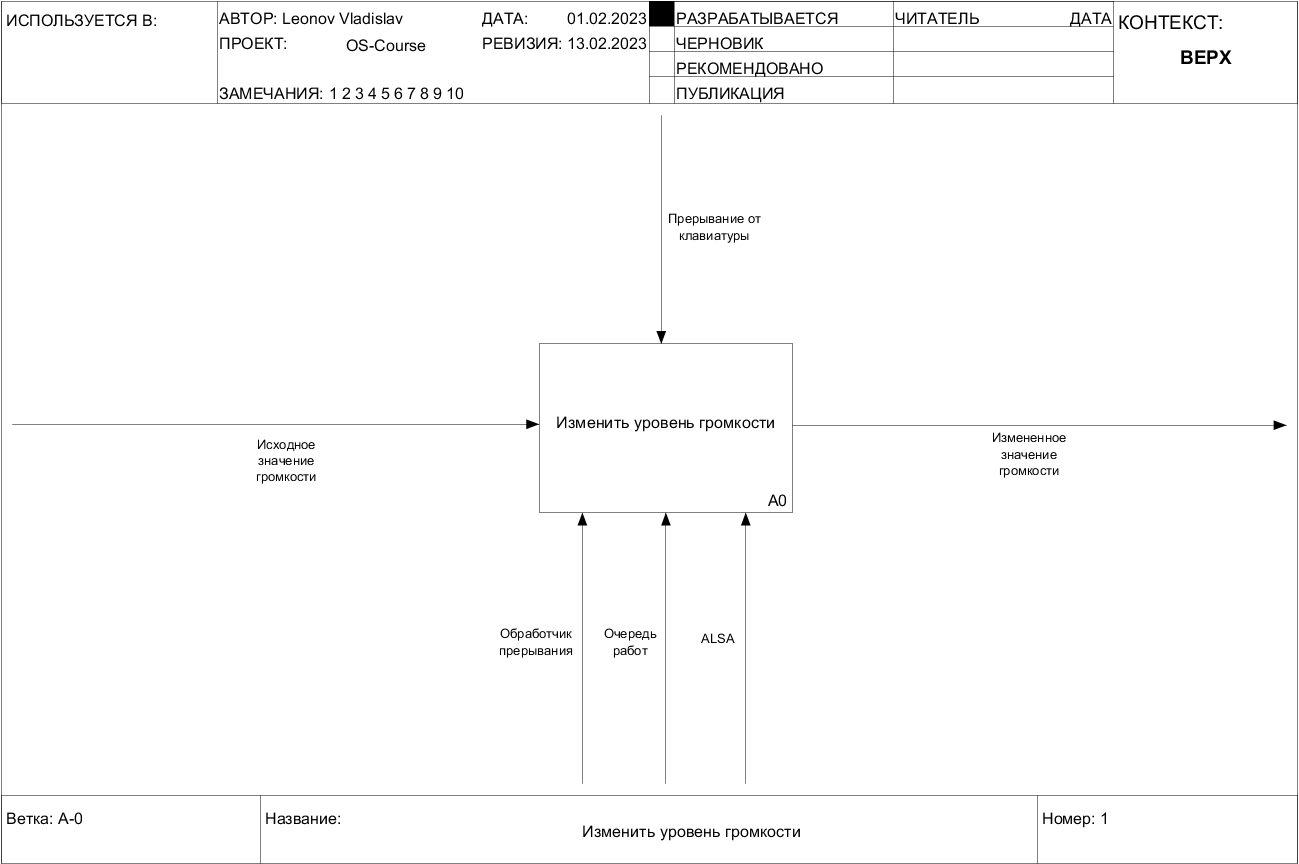
\includegraphics[scale = 0.35]{inc/img/01_A-0.png}
	\caption{Уровень А0}
	\label{fig:idef0-1}	
\end{figure}

\clearpage

\begin{figure}[h!btp]
	\centering
	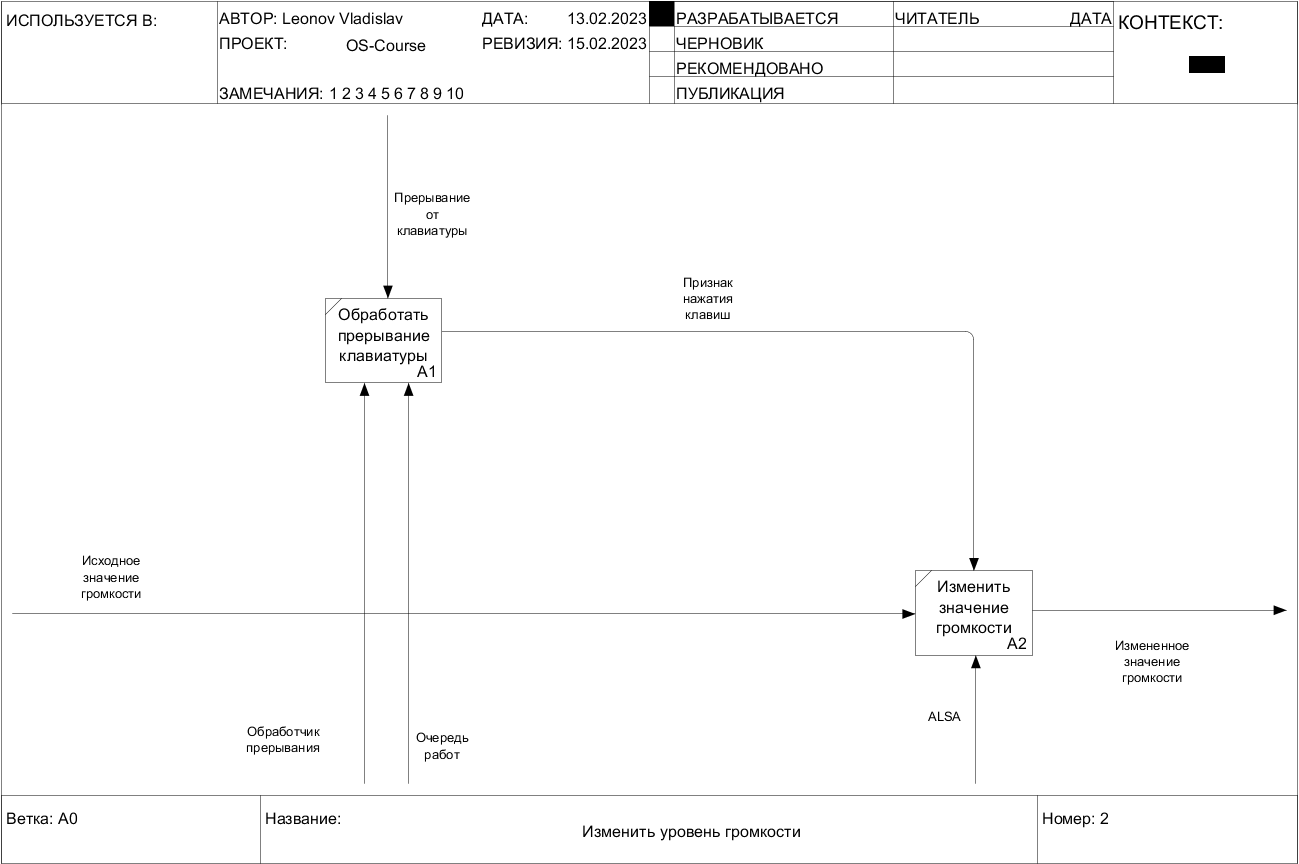
\includegraphics[scale = 0.35]{inc/img/02_A0.png}
	\caption{Уровень А1-A2}
	\label{fig:idef0-2}	
\end{figure}

\section{Разработка алгоритмов}

Одновременное нажатие следующих клавиш выполняет следующие действия:
\begin{itemize}
    \item ALT и 0 --- установить уровень громкости $0\%$; 
    \item ALT и 1 --- установить уровень громкости $10\%$; 
    \item ALT и 2 --- установить уровень громкости $20\%$; 
    \item ALT и 3 --- установить уровень громкости $30\%$; 
    \item ALT и 4 --- установить уровень громкости $40\%$; 
    \item ALT и 5 --- установить уровень громкости $50\%$; 
    \item ALT и 6 --- установить уровень громкости $60\%$; 
    \item ALT и 7 --- установить уровень громкости $70\%$; 
    \item ALT и 8 --- установить уровень громкости $80\%$; 
    \item ALT и 9 --- установить уровень громкости $90\%$; 
    \item ALT и -- --- уменьшить текущий уровень громкости на 1\%;
    \item ALT и = --- увеличить текущий уровень громкости на 1\%.     
\end{itemize}

Алгоритм обработки прерывания от клавиатуры изображен на рисунке \ref{fig:kb_handler}.
\begin{figure}[h!btp]
	\centering
	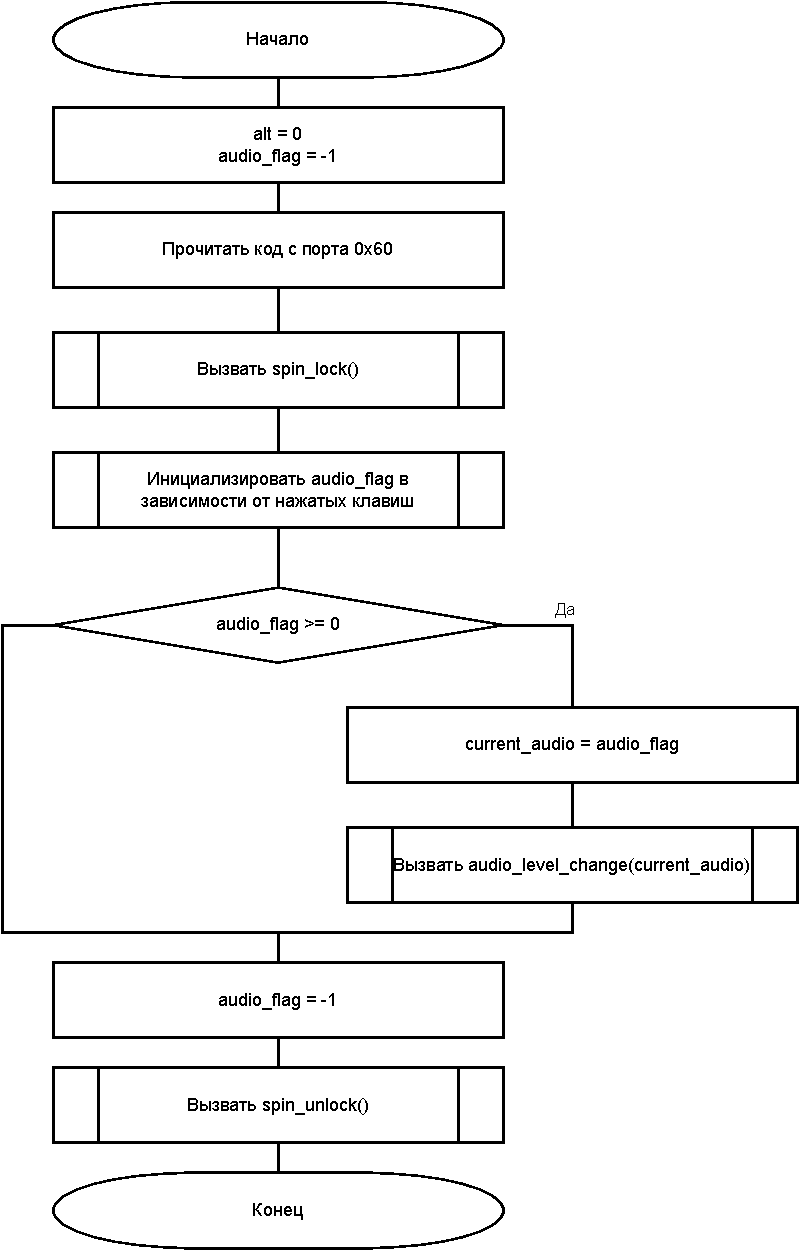
\includegraphics[scale = 0.9]{inc/diag/kb_handler.pdf}
	\caption{Алгоритм обработки прерывания от клавиатуры}
	\label{fig:kb_handler}	
\end{figure}

\clearpage

Алгоритм изменения громкости изображен на рисунке \ref{fig:volume_controller}.
\begin{figure}[h!btp]
	\centering
	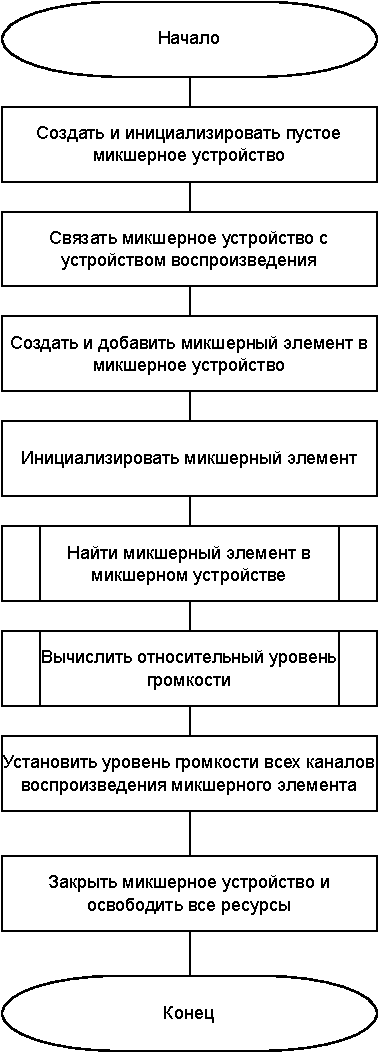
\includegraphics[scale = 1.3]{inc/diag/audio_controller.pdf}
	\caption{Алгоритм изменения громкости}
	\label{fig:volume_controller}	
\end{figure}

\clearpage

\section{Структура ПО}

Разработанное программное обеспечение включает в себя:
\begin{itemize}
    \item загружаемый модуль ядра, осуществляющий перехват прерываний от клавиатуры;
    \item вспомогательный модуль для регулировки громкости.
\end{itemize}

 На рисунке \ref{fig:module_struct} приведена структура ПО.
 \begin{figure}[h!btp]
	\centering
	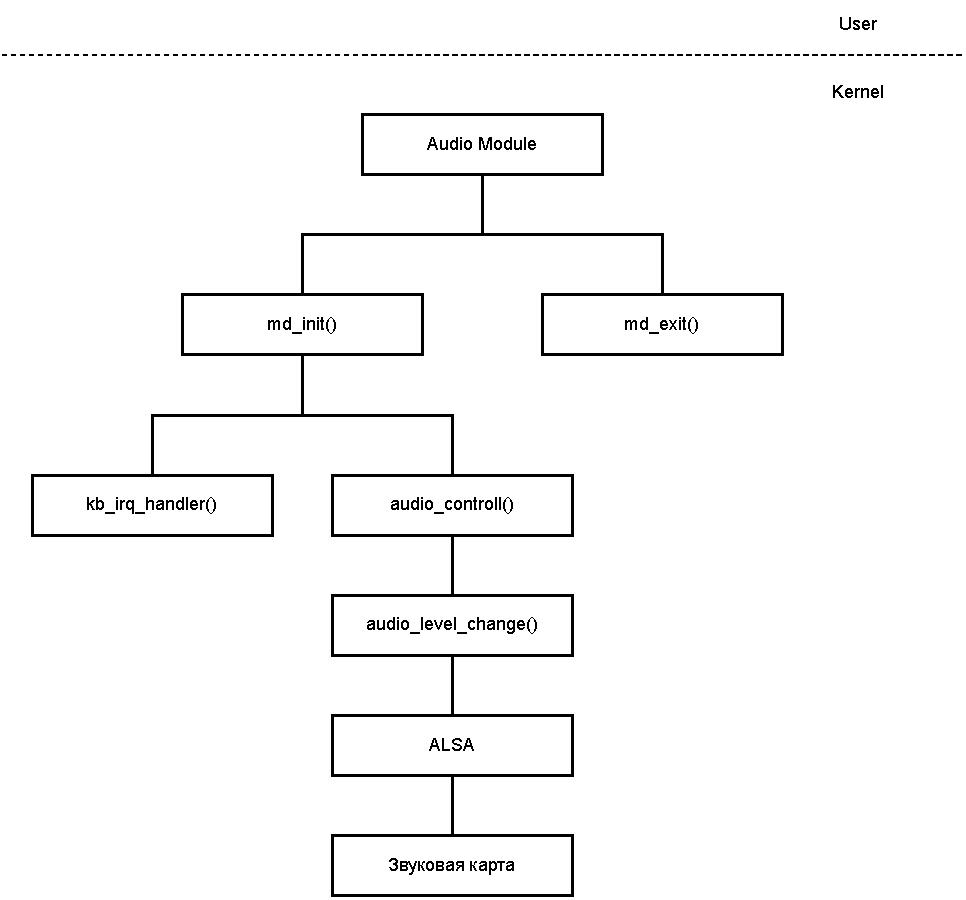
\includegraphics[scale = 1]{inc/diag/module_struct.pdf}
	\caption{Структура ПО}
	\label{fig:module_struct}	
\end{figure}


\chapter{Технологический раздел}

\section{Выбор языка и среды программирования}

В качестве языка программирования был выбран язык C. Данный ЯП используется для разработки всех модулей ядра и драйверов операционной системы Linux.

Среда программирования --- Microsoft Visual Studio Code \cite{vscode}. Данное решение является кроссплатформенным и бесплатным, а также имеет открытый исходный код.

\section{Точки входа в модуль}
В листингах \ref{lst:md_init}--\ref{lst:md_exit} представлены точки входа в модуль --- init и exit --- в которых происходит создание и уничтожение очереди работ, а также регистрация и дерегистрация обработчика прерываний от клавиатуры. 

\begin{lstlisting}[caption={Точки входа в модуль (часть 1)} \label{lst:md_init}]
static int __init md_init(void)
{
    int ret;
    printk(KERN_INFO "Module Initialization.\n");
    ret = request_irq(KB_IRQ, (irq_handler_t)kb_irq_handler, IRQF_SHARED, "Custom Handler", (void *)(kb_irq_handler));
    if (ret != 0)
        printk(KERN_INFO "Cannot Request IRQ for keyboard.\n");

    work = kmalloc(sizeof(struct work_struct), GFP_KERNEL);
    if (work)
    {
        INIT_WORK((struct work_struct *)work, audio_controll);
    }
    wq = create_workqueue("keyboard_queue");

    printk(KERN_INFO "Module Inited.\n");
    return 0;
}
\end{lstlisting}

\clearpage

\begin{lstlisting}[caption={Точки входа в модуль (часть 2)} \label{lst:md_exit}]
static void __exit md_exit(void)
{
    free_irq(KB_IRQ, (void *)(kb_irq_handler));
    flush_workqueue(wq);
    destroy_workqueue(wq);

    if (work)
        kfree(work);

    printk(KERN_INFO "Module Exit.");
}

module_init(md_init);
module_exit(md_exit);
\end{lstlisting}

\section{Обработка прерываний клавиатуры}
В листингах \ref{lst:kb_irq_handler}--\ref{lst:system_volume_control3} представлен обработчик прерываний клавиатуры.

\begin{lstlisting}[caption={Обработчик прерываний клавиатуры} \label{lst:kb_irq_handler}]
irq_handler_t kb_irq_handler(int irq, void *dev_id, struct pt_regs *regs)
{
    spin_lock(&k_lock);
    scancode = inb(0x60);
    spin_unlock(&k_lock);

    queue_work(wq, work);

    return (irq_handler_t)IRQ_HANDLED;
}
\end{lstlisting}

\begin{lstlisting}[caption={Обработчик нижней половины прерывания(часть 1)} \label{lst:system_volume_control1}]
void audio_controll(struct work_struct *work)
{
    static int alt = 0;
    static long audio_flag = -1;

    spin_lock(&k_lock);
    switch (scancode)
    {
    case ALT_PRESSED:
        alt = 1;
        break;
\end{lstlisting}

\clearpage

\begin{lstlisting}[caption={Обработчик нижней половины прерывания(часть 2)} \label{lst:system_volume_control2}]
    case ALT_UNPRESSED:
        alt = 0;
        break;
    case LEVEL0_PRESSED:
        if (alt)
            audio_flag = 0;
        break;
    case LEVEL1_PRESSED:
        if (alt)
            audio_flag = 10;
        break;
    case LEVEL2_PRESSED:
        if (alt)
            audio_flag = 20;
        break;
    case LEVEL3_PRESSED:
        if (alt)
            audio_flag = 30;
        break;
    case LEVEL4_PRESSED:
        if (alt)
            audio_flag = 40;
        break;
    case LEVEL5_PRESSED:
        if (alt)
            audio_flag = 50;
        break;
    case LEVEL6_PRESSED:
        if (alt)
            audio_flag = 60;
        break;
    case LEVEL7_PRESSED:
        if (alt)
            audio_flag = 70;
        break;
    case LEVEL8_PRESSED:
        if (alt)
            audio_flag = 80;
        break;
    case LEVEL9_PRESSED:
        if (alt)
            audio_flag = 90;
        break;
\end{lstlisting}

\clearpage

\begin{lstlisting}[caption={Обработчик нижней половины прерывания(часть 3)} \label{lst:system_volume_control3}]
    case LEVELMINUS_PRESSED:
        if (alt && current_audio > 0)
            audio_flag = current_audio - 1;
        break;
    case LEVELPLUS_PRESSED:
        if (alt && current_audio < 100)
            audio_flag = current_audio + 1;
        break;
    default:
        break;
    }

    if (audio_flag >= 0)
    {
        printk(KERN_INFO "System Volume Changing Started.\n");
        current_audio = audio_flag;
        char buffer[10];
        sprintf(buffer, "%d", current_audio);
        char *argv[] = {"/home/leerycorsair/os_course/audio_controller", buffer, NULL};
        static char *envp[] = {
            "HOME=/",
            "TERM=linux",
            "PATH=/sbin:/bin:/usr/sbin:/usr/bin", NULL};

        call_usermodehelper(argv[0], argv, envp, UMH_WAIT_PROC);
        printk(KERN_INFO "System Volume Changed to %d\%.\n", current_audio);
    }

    audio_flag = -1;
    spin_unlock(&k_lock);
}
\end{lstlisting}

\section{Функция изменения громкости}

В листинге \ref{lst:system_volume_controller} приведена структура, описывающая звуковое устройство для которого создается функция изменения громкости.

\clearpage

\begin{lstlisting}[caption={Структура system\_volume\_controller} \label{lst:system_volume_controller}]
struct audio_controller
{
    long min, max;
    snd_mixer_t *handle;
    snd_mixer_selem_id_t *sid;
    const char *card;
    const char *selem_name;
} a_controller;
\end{lstlisting}

В данной структуре созданы следующие поля:
\begin{itemize}
    \item min и max --- минимальный и максимальный физический уровень громкости;
    \item handle --- микшерное устройство;
    \item sid --- идентификатор микшерного элемента;
    \item card --- имя устройства воспроизведения;
    \item selem\_name --- имя микшерного элемента.
\end{itemize}

В листингах \ref{lst:system_volume_change1}--\ref{lst:system_volume_change2} представлена функция изменения уровня громкости.

\begin{lstlisting}[caption={Функция изменения громкости (часть 1)} \label{lst:system_volume_change1}]
void audio_level_change(long audio_level)
{
    a_controller.card = "default";
    a_controller.selem_name = "Master";

    if (snd_mixer_open(&(a_controller.handle), 0) < 0)
        return;

    if (snd_mixer_attach(a_controller.handle, a_controller.card) < 0)
        return;

    if (snd_mixer_selem_register(a_controller.handle, NULL, NULL) < 0)
        return;

    if (snd_mixer_load(a_controller.handle) < 0)
        return;

    snd_mixer_selem_id_alloca(&(a_controller.sid));
    snd_mixer_selem_id_set_index(a_controller.sid, 0);
    snd_mixer_selem_id_set_name(a_controller.sid, a_controller.selem_name);
\end{lstlisting}

\clearpage

\begin{lstlisting}[caption={Функция изменения громкости (часть 2)} \label{lst:system_volume_change2}]
    snd_mixer_elem_t *elem = snd_mixer_find_selem(a_controller.handle, a_controller.sid);
    if (elem == NULL)
        return;

    snd_mixer_selem_get_playback_volume_range(elem, &(a_controller.min), &(a_controller.max));
    if (snd_mixer_selem_set_playback_volume_all(elem, audio_level * a_controller.max / 100) < 0)
        return;

    snd_mixer_close(a_controller.handle);
}
\end{lstlisting}

\section{Сборка разработанного модуля}

Для компиляции загружаемого модуля используется утилита make. Конфигурационный файл makefile приведен в листинге \ref{lst:makefile} \cite{makefile}.

\begin{lstlisting}[caption={makefile для сборки} \label{lst:makefile}]
CONFIG_MODULE_SIG=n
CURRENT = $(shell uname -r)
KDIR = /lib/modules/$(CURRENT)/build
PWD = $(shell pwd)
TARGET = audio_module
obj-m := $(TARGET).o


default: audio_controller
	$(MAKE) -C$(KDIR) M=$(PWD) modules
  
audio_controller: audio_controller.c
	gcc -o $@ $@.c -lasound
\end{lstlisting}
\chapter{Исследовательский раздел}
\label{cha:research}

Для разработки и тестирования данной работы использовался ноутбук Honor MagicBook Pro 2021 и операционная система Linux Ubuntu 22.04. 

\section{Демонстрация последовательного изменения громкости}
На рисунке \ref{fig:module_steps} изображены логи последовательного изменения громкости.
\begin{figure}[h!btp]
	\centering
	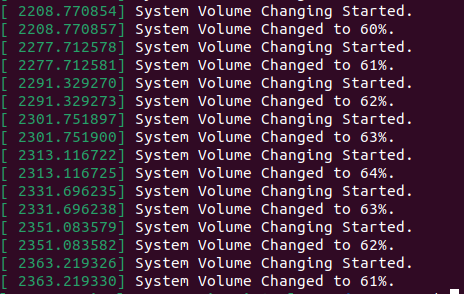
\includegraphics[scale = 1.3]{inc/img/module_steps.png}
	\caption{Логи последовательного изменения громкости}
	\label{fig:module_steps}	
\end{figure}

\clearpage

\section{Демонстрация использования заданной шкалы настроек}
На рисунке \ref{fig:module_levels} изображены логи при использовании заданной шкалы настроек громкости.

\begin{figure}[h!btp]
	\centering
	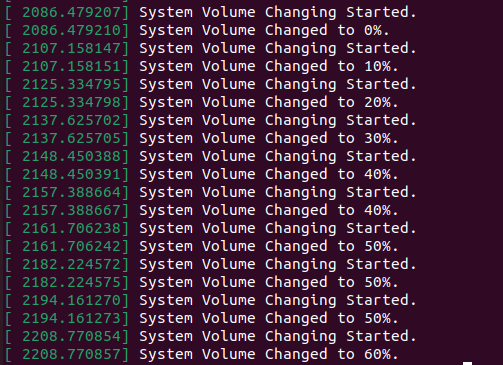
\includegraphics[scale = 1.25]{inc/img/module_levels.png}
	\caption{Логи при использовании заданной шкалы настроек громкости}
	\label{fig:module_levels}	
\end{figure}
\chapter*{ЗАКЛЮЧЕНИЕ}
\addcontentsline{toc}{chapter}{ЗАКЛЮЧЕНИЕ} 

В результате выполнения курсовой работы:
\begin{itemize}
    \item проанализированы способы обработки прерываний;
    \item проанализированы существующие аудио подсистемы;
    \item разработаны алгоритмы и описана структура разработанного ПО;
    \item разработано ПО, предоставляюшее заявленную функциональность;
    \item выполнено исследование разработанного ПО.
\end{itemize}

Таким образом, разработанное программное обеспечение отвечает поставленной задаче --- загружаемый модуль ядра Linux позволяет регулировать уровень громкости клавиатурой с возможностью использования заданной шкалы настроек.

\makebibliography

\begin{appendices}

\chapter{}
\begin{lstlisting}[caption={Листинг audio\_module.c(часть 1)}]
#include <linux/kernel.h>
#include <linux/module.h>
#include <linux/workqueue.h>
#include <linux/interrupt.h>
#include <linux/kmod.h>
#include <linux/slab.h>
#include <asm/io.h>

#define KB_IRQ 1

#define ALT_PRESSED 56    // Alt pressed
#define ALT_UNPRESSED 184 // Alt unpressed

#define LEVEL0_PRESSED 11     // Key 0 pressed 0%
#define LEVEL1_PRESSED 2      // Key 1 pressed 10%
#define LEVEL2_PRESSED 3      // Key 2 pressed 20%
#define LEVEL3_PRESSED 4      // Key 3 pressed 30%
#define LEVEL4_PRESSED 5      // Key 4 pressed 40%
#define LEVEL5_PRESSED 6      // Key 5 pressed 50%
#define LEVEL6_PRESSED 7      // Key 6 pressed 60%
#define LEVEL7_PRESSED 8      // Key 7 pressed 70%
#define LEVEL8_PRESSED 9      // Key 8 pressed 80%
#define LEVEL9_PRESSED 10     // Key 9 pressed 90%
#define LEVELMINUS_PRESSED 12 // Key - pressed decrease
#define LEVELPLUS_PRESSED 13  // Key = pressed increase

unsigned char scancode;
long current_audio = 0;

MODULE_LICENSE("GPL");
MODULE_AUTHOR("Leonov Vladislav");

DEFINE_SPINLOCK(k_lock);

static struct workqueue_struct *wq;
static struct work_struct *work;   
\end{lstlisting}
\clearpage


\begin{lstlisting}[caption={Листинг audio\_module.c(часть 2)}]
void audio_controll(struct work_struct *work)
{
    static int alt = 0;
    static long audio_flag = -1;

    spin_lock(&k_lock);
    switch (scancode)
    {
    case ALT_PRESSED:
        alt = 1;
        break;
    case ALT_UNPRESSED:
        alt = 0;
        break;
    case LEVEL0_PRESSED:
        if (alt)
            audio_flag = 0;
        break;
    case LEVEL1_PRESSED:
        if (alt)
            audio_flag = 10;
        break;
    case LEVEL2_PRESSED:
        if (alt)
            audio_flag = 20;
        break;
    case LEVEL3_PRESSED:
        if (alt)
            audio_flag = 30;
        break;
    case LEVEL4_PRESSED:
        if (alt)
            audio_flag = 40;
        break;
    case LEVEL5_PRESSED:
        if (alt)
            audio_flag = 50;
        break;
    case LEVEL6_PRESSED:
        if (alt)
            audio_flag = 60;
        break;
    case LEVEL7_PRESSED:
        if (alt)
            audio_flag = 70;
        break;
\end{lstlisting}

\clearpage

\begin{lstlisting}[caption={Листинг audio\_module.c(часть 3)}]
    case LEVEL8_PRESSED:
        if (alt)
            audio_flag = 80;
        break;
    case LEVEL9_PRESSED:
        if (alt)
            audio_flag = 90;
        break;
    case LEVELMINUS_PRESSED:
        if (alt && current_audio > 0)
            audio_flag = current_audio - 1;
        break;
    case LEVELPLUS_PRESSED:
        if (alt && current_audio < 100)
            audio_flag = current_audio + 1;
        break;
    default:
        break;
    }

    if (audio_flag >= 0)
    {
        printk(KERN_INFO "System Volume Changing Started.\n");
        current_audio = audio_flag;
        char buffer[10];
        sprintf(buffer, "%d", current_audio);
        char *argv[] = {"/home/leerycorsair/os_course/audio_controller", buffer, NULL};
        static char *envp[] = {
            "HOME=/",
            "TERM=linux",
            "PATH=/sbin:/bin:/usr/sbin:/usr/bin", NULL};

        call_usermodehelper(argv[0], argv, envp, UMH_WAIT_PROC);
        printk(KERN_INFO "System Volume Changed to %d\%.\n", current_audio);
    }

    audio_flag = -1;
    spin_unlock(&k_lock);
}

irq_handler_t kb_irq_handler(int irq, void *dev_id, struct pt_regs *regs)
{
    spin_lock(&k_lock);
    scancode = inb(0x60);
    spin_unlock(&k_lock);
\end{lstlisting}

\clearpage

\begin{lstlisting}[caption={Листинг audio\_module.c(часть 4)}]
    queue_work(wq, work);

    return (irq_handler_t)IRQ_HANDLED;
}

static int __init md_init(void)
{
    int ret;
    printk(KERN_INFO "Module Initialization.\n");
    ret = request_irq(KB_IRQ, (irq_handler_t)kb_irq_handler, IRQF_SHARED, "Custom Handler", (void *)(kb_irq_handler));
    if (ret != 0)
        printk(KERN_INFO "Cannot Request IRQ for keyboard.\n");

    work = kmalloc(sizeof(struct work_struct), GFP_KERNEL);
    if (work)
    {
        INIT_WORK((struct work_struct *)work, audio_controll);
    }
    wq = create_workqueue("keyboard_queue");

    printk(KERN_INFO "Module Inited.\n");
    return 0;
}

static void __exit md_exit(void)
{
    free_irq(KB_IRQ, (void *)(kb_irq_handler));
    flush_workqueue(wq);
    destroy_workqueue(wq);

    if (work)
        kfree(work);

    printk(KERN_INFO "Module Exit.");
}

module_init(md_init);
module_exit(md_exit);
\end{lstlisting}

\clearpage

\begin{lstlisting}[caption={Листинг audio\_controller.c}]

#include <alsa/asoundlib.h>

struct audio_controller
{
    long min, max;
    snd_mixer_t *handle;
    snd_mixer_selem_id_t *sid;
    const char *card;
    const char *selem_name;
} a_controller;

void audio_level_change(long audio_level)
{
    a_controller.card = "default";
    a_controller.selem_name = "Master";

    if (snd_mixer_open(&(a_controller.handle), 0) < 0)
        return;

    if (snd_mixer_attach(a_controller.handle, a_controller.card) < 0)
        return;

    if (snd_mixer_selem_register(a_controller.handle, NULL, NULL) < 0)
        return;

    if (snd_mixer_load(a_controller.handle) < 0)
        return;

    snd_mixer_selem_id_alloca(&(a_controller.sid));
    snd_mixer_selem_id_set_index(a_controller.sid, 0);
    snd_mixer_selem_id_set_name(a_controller.sid, a_controller.selem_name);

    snd_mixer_elem_t *elem = snd_mixer_find_selem(a_controller.handle, a_controller.sid);
    if (elem == NULL)
        return;

    snd_mixer_selem_get_playback_volume_range(elem, &(a_controller.min), &(a_controller.max));
    if (snd_mixer_selem_set_playback_volume_all(elem, audio_level * a_controller.max / 100) < 0)
        return;

    snd_mixer_close(a_controller.handle);
}
\end{lstlisting}


\end{appendices}

\end{document}